\documentclass{thesisclass}
% Based on thesisclass.cls of Timo Rohrberg, 2009
% ----------------------------------------------------------------
% Thesis - Main document
% ----------------------------------------------------------------
% No empty in-between chapters, remove this line if desired for double-page printing
\let\cleardoublepage\clearpage

% you can add custom packages that you may need
\usepackage{amsmath}
\usepackage{hyperref}
\usepackage[acronym]{glossaries}

\makenoidxglossaries

\newacronym{dof}{DoF}{depth of field}

\newacronym{mb}{MB}{motion blur}

\newacronym{coc}{CoC}{circle of confusion}

\newacronym{psf}{PSF}{point spread function}

\newacronym{lerp}{lerp}{linear interpolation}

\newacronym{lerping}{lerping}{inerpolating linearly}


%% -------------------------------
%% |  Information for PDF file   |
%% -------------------------------
\hypersetup{
 pdfauthor={Fabian Zürker Aguilar},
 pdftitle={Simulation of camera artefacts in real-time applications},
 pdfsubject={Not set},
 pdfkeywords={Not set}
}


%% ---------------------------------
%% | Information about the thesis  |
%% ---------------------------------

\newcommand{\myname}{Fabian Zürker Aguilar}
\newcommand{\mytitle}{Simulation of camera artefacts in real-time applications}
\newcommand{\myinstitute}{Institut für Visualisierung und Datenanalyse,\\ Lehrstuhl für Computergrafik}

\newcommand{\reporttype}{Proseminar}                                  % Proseminar-/Seminar-/Bachelor-/Master
%\newcommand{\reviewerone}{Prof. Dr.-Ing. Carsten Dachsbacher}     % only for bachelor/master
%\newcommand{\reviewertwo}{Prof. Dr. Hartmut Prautzsch}            % only for bachelor/master
\newcommand{\advisorone}{Max Piochowiak}
%\newcommand{\advisortwo}{?}                                      % only if applicable

\newcommand{\timestart}{XX. Monat 20XX}
\newcommand{\timeend}{XX. Monat 20XX}
\newcommand{\submissiontime}{DD. MM. 20XX}


%% ---------------------------------
%% | ToDo Marker - only for draft! |
%% ---------------------------------
% Remove this section for final version!
\setlength{\marginparwidth}{20mm}

\newcommand{\margtodo}
{\marginpar{\textbf{\textcolor{red}{ToDo}}}{}}

\newcommand{\todo}[1]
{{\textbf{\textcolor{red}{(\margtodo{}#1)}}}{}}


%% --------------------------------
%% | Old Marker - only for draft! |
%% --------------------------------
% Remove this section for final version!
\newenvironment{deprecated}
{\begin{color}{gray}}
{\end{color}}


%% --------------------------------
%% | Settings for word separation |
%% --------------------------------
% Help for separation:
% In german  the following hints are additionally available:
% "- = Additional separation
% "| = Suppress ligation and possible separation (e.g. Schaf"|fell)
% "~ = Hyphenation without separation (e.g. bergauf und "~ab)
% "= = Hyphenation with separation before and after
% "" = Separation without a hyphenation (e.g. und/""oder)

% Describe separation hints here:
\hyphenation{
% Pro-to-koll-in-stan-zen
% Ma-na-ge-ment  Netz-werk-ele-men-ten
% Netz-werk Netz-werk-re-ser-vie-rung
% Netz-werk-adap-ter Fein-ju-stier-ung
% Da-ten-strom-spe-zi-fi-ka-tion Pa-ket-rumpf
% Kon-troll-in-stanz
}


%% ------------------------
%% |    Including files   |
%% ------------------------
% Only files listed here will be included!
% Userful command for partially translating the document (for bug-fixing e.g.)
\includeonly{%
titlepage,
content,
}


%%%%%%%%%%%%%%%%%%%%%%%%%%%%%%%%%
%% Here, main documents begins %%
%%%%%%%%%%%%%%%%%%%%%%%%%%%%%%%%%
\begin{document}

% Remove the following line for German text
%\selectlanguage{ngerman}
\selectlanguage{english}

\frontmatter
\pagenumbering{roman}
%% titlepage.tex
%%

% coordinates for the bg shape on the titlepage
\newcommand{\diameter}{20}
\newcommand{\xone}{-15}
\newcommand{\xtwo}{160}
\newcommand{\yone}{15}
\newcommand{\ytwo}{-253}

\newcommand{\checkfor}[2]{%
  \ifcsname#1\endcsname%
    #2
  \fi%
}

\begin{titlepage}
% bg shape
\begin{tikzpicture}[overlay]
\draw[color=gray]  
 		 (\xone mm, \yone mm)
  -- (\xtwo mm, \yone mm)
 arc (90:0:\diameter pt) 
  -- (\xtwo mm + \diameter pt , \ytwo mm) 
	-- (\xone mm + \diameter pt , \ytwo mm)
 arc (270:180:\diameter pt)
	-- (\xone mm, \yone mm);
\end{tikzpicture}
	\begin{textblock}{10}[0,0](4,2.5)
		
\includegraphics[width=.3\textwidth]{logos/KITLogo_RGB.pdf}
	\end{textblock}
	\changefont{phv}{m}{n}	% helvetica	
	\vspace*{3.5cm}
	\begin{center}
		\Huge{\mytitle}
		\vspace*{2cm}\\
		\Large{
      \reporttype\iflanguage{english}{ Thesis of}{-Ausarbeitung von}
		}\\
		\vspace*{1cm}
		\huge{\myname}\\
		\vspace*{1cm}
		\Large{
      \iflanguage{english}{At the Department of Informatics}{An der Fakult\"at f\"ur Informatik}
			\\
			\myinstitute
		}\\
		\vspace*{1cm}
		\Large{\today}
	\end{center}
	\vspace*{1cm}
\Large{
\begin{center}
\begin{tabular}[ht]{l c l}
  % Gutachter sind die Professoren, die die Arbeit bewerten. 
  \checkfor{reviewerone}{\iflanguage{english}{Reviewer}{Erstgutachter}: & \hfill  & \reviewerone}\\
  \checkfor{reviewertwo}{\iflanguage{english}{Second reviewer}{Zweitgutachter}: & \hfill  & \reviewertwo}\\
  \checkfor{advisorone}{\iflanguage{english}{Advisor}{Betreuender Mitarbeiter}: & \hfill  & \advisorone}\\
  \checkfor{advisortwo}{\iflanguage{english}{Second advisor}{Zweiter betreuender Mitarbeiter}: & \hfill  & \advisortwo}\\
  % Der zweite betreuende Mitarbeiter kann weggelassen werden. 
\end{tabular}
\end{center}
}


\vspace{2cm}


\begin{textblock}{10}[0,0](4,16.8)
\tiny{ 
  \iflanguage{english}{KIT -- The Research University in the Helmholtz Association}{KIT -- Die Forschungsuniversität in der Helmholtz-Gesellschaft}
}
\end{textblock}

\begin{textblock}{10}[0,0](14,16.75)
\large{
	\textbf{www.kit.edu} 
}
\end{textblock}

\end{titlepage}

\blankpage

\chapter*{Abstract}
With the rapid advance in computer graphics in various application like video games, virtual reality and augmented reality, the generation of immersive real-time images has become a critical component of these future systems.
To increase immersiveness of the application it is critical to also recreate the flaws of the human eye or camera systems.
However, a realistic simulation of the optical system of a camera is currently outside the scope of real-time images.
We explore a range of techniques to approximate artifacts of a camera system that are expected by a viewer in cinematic contexts.
These techniques are applicable in a wide range of application ranging from mobile virtual reality to video games played on a computer or console.

%% -------------------
%% |   Directories   |
%% -------------------
\tableofcontents
\blankpage


%% -----------------
%% |   Main part   |
%% -----------------
\mainmatter
\pagenumbering{arabic}
%% content.tex
%%
\chapter{Introduction}
\label{ch:Introduction}


\chapter{Background on camera systems}
\label{ch:background}
Most real-time renderers use the simple pinhole camera model to create their images.
This approach leads to perfect images of the scene at a moment in time.
However to achieve a more realistic image or an artistic vision these images are to perfect, as they do not express real visual artefacts cameras and human eyes experience.
\section{Lens and aperture}
\label{ch:background-lens}
The simplest camera model is the pinhole camera.
An infinitesimal small hole is punched into an opaque material and creates the aperture.
An image is then taken from an image plane places at distance $d$ parallel to the aperture.
This camera model can be implemented easily in computer graphics software by modeling the aperture as a singe point in space.
The incoming light is then approximated by a ray emanating at an object or light source and crossing the aperture point.
This ray then intersects the image plane of the virtual camera at a single point and a color value is recorded.
This procedure is typically reversed for actual graphics pipelines with rays coming emanating at predetermined points on the image plane and crossing the aperture point.

If the aperture of a pinhole camera is assumed to be an infinitesimally small hole i.e. a point in space and light is approximated by straight rays, then the pinhole camera represents the ideal perspective camera.
Each point on the image plane only receives light from exactly one point and is therefore perfectly in focus.
The camera can therefore be described as a coordinate transformation $x_c, y_c, z_c \mapsto x, y$.
The resulting image coordinates $x, y$ can be derived from the equations:
\begin{align}
    \frac{x_c}{x} = -\frac{z_c}{d} \\
    \frac{y_c}{y} = -\frac{z_c}{d}
\end{align}
This results in the following projection:
\begin{align}
    \begin{pmatrix}
    x_c \\
    y_c \\
    z_c
\end{pmatrix} 
\mapsto
\begin{pmatrix}
    x \\
    y
\end{pmatrix}
= -\frac{d}{z_c}
\begin{pmatrix}
    x_c \\
    y_c
\end{pmatrix}
\end{align}
The negative sign represents the flipping of the image on the image plane \cite{Beyerer.2016}.

In reality this camera model suffers from multiple issues that make pinhole cameras unpractical for photography.
The most obvious problem is the impossibility to create a infinitesimally small hole.
Consequently, the aperture will always have a real diameter $A > 0$.
This causes a point on the image plane to receive light from multiple sources and thus negates the theoretically perfect focus of the pinhole camera.
If one still tries to approach a $A$ of $0$ the light entering the pinhole will also approach $0$.
The image will become darker or the exposure time needed for a bright image will approach infinity.
Additionally at such small values of $A$ the assumption of light as a ray will break down and one will notice diffraction start to appear and blurring the image further \cite{Beyerer.2016}.

\begin{figure}[h]
    \centering
    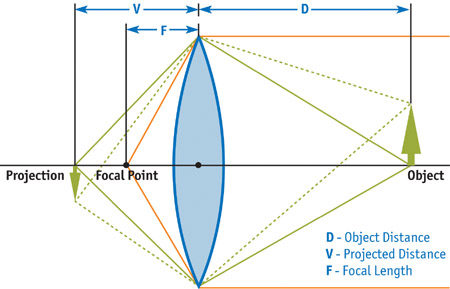
\includegraphics[width=0.8\textwidth]{images/fig23-01_1.png}
    \caption{Optical mapping of a thin-lens}
    \label{fig:thin-lens}
    \cite{Demers.2005}
\end{figure}

To increase the amount of light hitting the image plane one or more lenses are used in real camera systems.
In the following we will only describe single thin-lens system, as they are sufficient to demonstrate the most important visual phenomena.
Lenses are used to bundle all light entering parallel to the optical axis at the focal point of the lens.
The relation between the radius of the lens $R$ and the distance of the focal point $F$ to the lens can be described as
\begin{align}
    R = 2 F \frac{n_2 - n_1}{n_1}
\end{align}
with $n_1$ representing the refractive index of the surrounding material and $n_2$ the refractive index of the lens \cite{Beyerer.2016}.

Most lens system are constructed with rotational symmetry with the light entering at small angles $\alpha$ between the light ray and the optical axis.
As such the approximation $\sin  \alpha \approx \alpha$ holds and we can linearize the law of refraction to
\begin{align}
    n_1 \sin \theta_1 = n_2 \sin \theta_2 \rightarrow n_1 \theta_1 = n_2 \theta_2.
\end{align}
This approximation is called paraxial approximation and enables the modeling of spherical lenses as linear systems with their associated matrices. \cite{Beyerer.2016}

The relation between the object and image can be described with
\begin{align}
    \frac{1}{F} &= \frac{1}{D} + \frac{1}{V} \\
    \frac{Size\:of\:object}{F} &= -\frac{Size\:of\:image}{V-F}.
    \label{eq:sharp-thin-lens}
\end{align}

As such the \gls{dof} of a camera with a distance is limited to a single plane with distance $P$.

\begin{figure}[h]
    \centering
    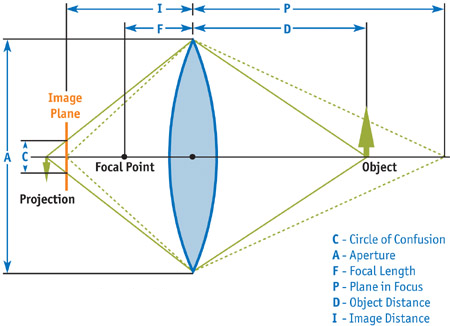
\includegraphics[width=0.8\textwidth]{images/fig23-02_1.png}
    \caption{Thin lens with imperfect focus}
    \label{fig:coc-thin-lens}
    \cite{Demers.2005}
\end{figure}
However a perfectly sharp image is not necessary as an image sensor cannot resolve details smaller than a certain size.
This lower limit is typically given by the physical size of the sensor pixels.
We therefore have a range of values of $D$ such that the image still appears in focus.
Using similar triangles we can derive the equation
\begin{align}
    \frac{C}{A} = \frac{D-I}{D} \implies C = A \cdot |\frac{D-I}{D}|.
    \label{eq:coc}
\end{align}
To have more control over the camera, the equation can be expanded to:
\begin{align}
    C = | A \cdot \frac{F(P-D)}{D(P-F)}|.
    \label{eq:coc-expanded}
\end{align}
$C$ describes the radius of the image a single dot on the image plane and is called \gls{coc}.
This equation can be used to derive the following equation for \gls{dof}:
\begin{align}
    |P-D| = |P-D|(A) = \frac{C \cdot D}{\frac{A F}{P-F} - C}
    \label{eq:dof}
\end{align}
A few notes on equation \ref{eq:coc} and \ref{eq:dof}:
\begin{itemize}
    \item Pinhole cameras have a diameter $A$ of 0 and thus perfect focus. Any real lens, including the human eye has a $A$ greater than 0.
    \item To increase the \gls{dof} $A$ is typically reduced by the use of an aperture at the expense of image brightness.
    \item The \gls{coc} increases much faster in the foreground than in the background.
\end{itemize}

The blur of optical system can be described by its \gls{psf}.
It characterizes the spread of a single point source of light onto the image plane and takes into account the many factors that contribute to a blurring of the image.
This includes, but is not limited to, imperfections in the lens, the shape of the aperture, diffraction effects and spherical and chromatic aberrations.
The \gls{psf} is typically represented as a two-dimensional function with a Gaussian or disk-like shape.
When thinking of an optical system as a function $f$ that transform incoming light rays into an image, the \gls{psf} represents its impulse response function \cite{Beyerer.2016}.
The ability to define the particular \gls{psf} used is important to simulate particular camera systems accurately.

\begin{figure}
    \centering
    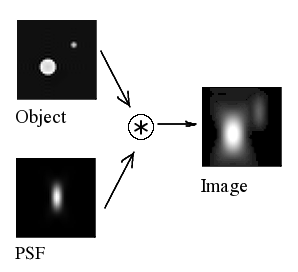
\includegraphics[width=0.6\textwidth]{images/Convolution_Illustrated_eng.png}
    \caption{Light source convoluted with \gls{psf} \cite{psf}}
    \label{fig:psf}
\end{figure}

\section{Sensor}
In contrast to a virtual camera an image sensor cannot interrogate the color of an object, but must wait for light to hit its light sensors and produce a strong enough image.
During the capture of a frame the view of a point camera can be described by
\begin{align}
    I(\omega) = \int_{\Delta T} f(\omega,t) L(\omega,t)dt.
    \label{eq:mb-integral}
\end{align}
Where $\omega$ is the direction of the incoming light, $L(\omega,t)$ is the incoming radiance and $f(\omega,t)$ models the influence of the optical system.
This equation can be adjusted to be more applicable to computer-graphics systems as
\begin{align}
    I_{xy} = \sum_l \int_\Omega \int_{\Delta T} f(\omega, t) g_l(\omega, t) L_l(\omega, t) \: dt \: d\omega.
    \label{eq:mb-cg-integral}
\end{align}
Here the pair $(x,y)$ represent the coordinates of the image pixel.
The geometry of each object is accounted for by iterating over all objects $l$.
To also account for the occlusion of objects in the scene $g_l(\omega, t)$ that is 1 if the object $l$ is directly visible and 0 if not.
Even though $g_l(\omega, t)$ does not account for transparent or reflective objects, this is not a limitation of the model as the term $L_l(\omega, t)$ accounts for these situations.
$L_l(\omega, t)$ simply describes what light is coming from angle $\Omega$ at time $t$ without describing the method how this is achieved. \cite{Navarro.2011}
For any computer-generated images the renderer must approximate this integral.

The effects of motion blur are often unwanted, especially in photography, and are reduced with lowering the exposure time of the image sensor.
This leaves less time for light to enter the sensor and therefore reduces image brightness.
To compensate for this either the sensitivity of the sensor (ISO) must be increased or the aperture must be widened to increase the amount of light entering.
Both options come with trade-offs to image quality.
Increasing the sensor sensitivity also introduces noise to the final image, while increasing the aperture diameter reduces the \gls{dof} (see equation \ref{eq:dof}).

% only digital image sensors considered
% sensors are exposed for a fixed length of time for each image
% longer time increases brightness but causes blurring of moving objects
% low brightness can be compensated with higher iso at cost of higher noise
% sensors can be exposed all at once or one line at a time
% bright light spills over into neighbouring pixels (bloom)
% pixels are layed out in special patterns  (beyer)
% the color of a pixel in a frame can be described as an integral over all angels over the exposure time

\chapter{Depth-of-Field}
As discussed in chapter \ref{ch:background} virtual cameras are able to take perfect color samples from every angle and thus create an image with infinite depth-of-field.
However without expensive operations, like the simulation of a lens with path tracing, a virtual camera is only able to create perfect images.
As such the difficulty in simulating depth of field in real-time lies in combining images with infinite depth of field into good approximation of real camera images.
\section{Accumulation buffers}
The image is rendered multiple times.
Each time shifting the virtual camera to simulate the circle of confusion (CoC).
The image around the point on which the camera is pointed moves very little thus creating very little blur.
The image far away from the focus point differ wildly and therefore are very blurred.
Workload is increased n-fold. Converges to correct answer

\section{2.5 dimensional rendering}
Render background blurred.
Render objects in focus.
Render foreground blurred.

Object can't go between layers.
background and foreground are uniformly blurred, without variation with distance.

\section{Backwards depth mapping}
z-buffer is generated with image.

Simple form: Each pixel is blurred according to distance from focus plane.
But: Generates unrealistic result at the boundaries of object with far background.

% Depth-of-Field Rendering by Pyramidal Image Processing
% https://onlinelibrary.wiley.com/doi/abs/10.1111/j.1467-8659.2007.01088.x
Complex form: Split image into n sub-images, culling pixels not in same "plane".
Culled pixels are disoccluded with chosen method and each sub-image is blurred according to distance to focus distance.
Images are combined to create final image.



\chapter{Motion blur}
\label{ch:mb}
In the vast majority of real-world applications, neither the camera nor the scene remain stationary.
A static snapshot of the scene, therefore, fails to capture any motion taking place.
Consequently, rapid motion in the scene or of the camera cannot be accurately represented without increasing the frame rate.
This lack of representation results is temporal aliasing between frames, which is jarring and disorienting for the viewer.
This effect is particularly exacerbated in interactive applications as there is no control of the camera.
As such multiple approaches to reduce temporal aliasing, in application where computational resources and thus frame rates are limited, have been developed.

\section{Accumulation buffers}
\label{ch:mb-acc}
The closest approximation of motion blur using traditional rendering pipelines can be achieved by the use of accumulation buffers.
This method is relatively easy to understand and implement.
A hardware buffer is used to average over $N$ rendering passes at different time steps.
The equation \ref{eq:mb-cg-integral} is approximated as

\begin{align}
    I_{xy} \approx \sum_{i=0}^{N-1} \frac{1}{N} \sum_{l} \int_\Omega f(\omega, t_i) g_l(\omega, t_i) L_l(\omega, t_i) \: d\omega.
\end{align}

Each individual frame is added with a factor of $\frac{1}{N}$, but these factors can be adjusted if a particular effect is desired.
With higher values of $N$ this method approaches the correct solution, but only displays a new image every $N$ rendering passes.
In many application this results in an unacceptable loss of performance \cite{Haeberli.1990}.

If higher update rates are desired and all frames are added with the same factor, filtering by repeated integration can be used \cite{Heckbert.1986}.
Initially $N$ frames are rendered normally and the resulting image is displayed.
To generated the next image, the first frame is rendered again and subtracted from the accumulation buffer.
Then frame $N+1$ is rendered and added to the accumulation buffer.
With this method a new image is displayed for every two frames rendered \cite{Haeberli.1990}.

%If more memory space and bandwidth are available, one can also choose to keep each image in a separate buffer and overwrite the oldest each rendering pass.
%The final image is then calculated using blending over all frames.
%This approach trades off the multiple rendering passes for an increase in memory utilization.

\section{Geometry substitution}
\label{ch:mb-gs}
An alternative approach to reduce temporal aliasing by increasing the frame rate involves modifying the underlying geometry to approximate a moving object.
The geometry and its texture are "smeared" across multiple time steps, while only one image is captured.
These methods work by approximating the equation \ref{eq:mb-cg-integral} to 

\begin{align}
    I_{xy} \approx \sum_{l'} \int_\Omega r_s(\omega)g_{l'}'(\omega)L_{l'}'(\omega) \: d\omega
    \label{eq:mb-geo-approx}
\end{align}

In equation \ref{eq:mb-geo-approx} the geometry $l$ is replaced by an alternative geometry $l'$ and all other functions are replaced by time-independent replacements.
As such this approach can referred to as a geometry post-processing effect, because it operates in object rather than in image space.

The first method implementing this approach was presented by Wloka et al. \cite{Wloka.1996} and demonstrates the basic method.
Their method begins by calculating the motion vector of an objects motion relative to the camera using the equation

$$
v_{obj} = (pos_{cam}(t_1) - pos_{cam}(t_0)) - (pos_{obj}(t_1) - pos_{obj}(t_0).
$$

This vector is then transformed to object space to operate on the object.
For the linear movement between the timesteps $t_0$ and $t_1$, $v_{obj}$ defines a front and back half of the object:

\begin{align}
    FrontPolygons &= \{ p |  Normal(p) \cdot v_{obj} \geq 0 \} \\
    BackPolygons  &= \{ p |  Normal(p) \cdot v_{obj} < 0 \}.
\end{align}

To ensure coherency and of the resulting motion volume, the object at timestep $t_1$ is used in the following steps.
The back half of polygons are moved by $-v_{obj}$ to the starting position of the motion and connected to the front half, as illustrated in figure \ref{fig:object-splitting}.
Alternatively, the transformation matrix, of the previous frame, is used for $FrontPolygons$ and the current transformation matrix for $BackPolygons$.

\begin{figure}[h]
    \centering
    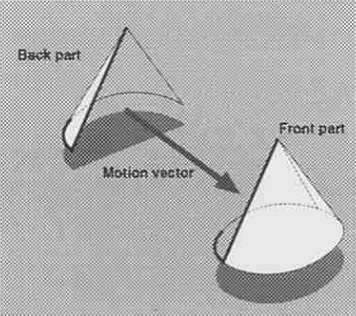
\includegraphics[width=0.4\textwidth]{images/object-splitting.png}
    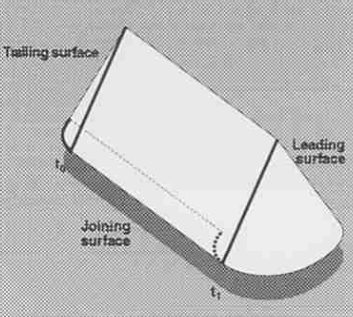
\includegraphics[width=0.4\textwidth]{images/object-splitting-assembly.png}
    \caption{Disassembly of object and construction of motion volume \cite{Wloka.1996}}
    \label{fig:object-splitting}
\end{figure}

Finally the transparency of the resulting motion volume is varied across its length to simulate a convincing motion blur.
A variety of functions are available to the artist to simulate different accelerations or shutters.
To represent non-linear motion the joining surface may be split at additional points to approximate curves \cite{Wloka.1996}.

Since this method can be executed by the vertex shader, its performance is very high.
However, the basic implementation of this approach comes with various limitation that preclude its use in modern applications.
The most significant constraints include the missing support for polygons with genus higher than zero (i.e., a torus) and rotation.
Additionally any real-time shadows calculated for the moving object must consider the transparency added to the motion volume by its motion.
Nevertheless, this simple method plays an important part in the approach discussed in section \ref{ch:mb-mf}.

\section{Motion fields}
\label{ch:mb-mf}
Motion fields provide another method to alleviate temporal aliasing, using the concept of vector fields to represent motion in the scene.
Similar to depth fields, motion fields supply additional information to image space algorithms by capturing the direction and magnitude of movement in the scene.

The basic idea behind motion fields is to record the motion vector in screen space at every pixel in the image for the duration of a frame.
This is accomplished in a vertex shader by transforming each vertex to window coordinates using the current and previous transformation matrix.
This results in two 2D-vectors $(x_s,y_s)$ and $(x_d,y_d)$ for the source and destination coordinates of a vertex.
The resulting movement vector of $(x_r,y_r) = (x_d - x_s,y_d - y_s)$ can be used directly or divided by $dt$ to get the screen space velocity.

The recorded motion field can then be used in several ways.
One straightforward application is to interpolate it across the geometry and pass that information to the pixel shader.
It would then 'smear' the image along the motion vectors, simulating a type of motion blur.
This can be mathematically represented as:

\begin{align}
    I_{xy} &= \frac{1}{N} \sum_{i=0}^{N-1}  S(x_s + x_r \frac{i}{N-1}, y_s + y_r \frac{i}{N-1}),
    \label{eq:mb-mf-approx}
\end{align}
where $S$ represents the rendered starting image.
Again the factors of $1/N$ may be adjusted to other filters (e.g. Gaussian or ramp) to simulate different types of motion.

This simple approach can be done in a single rendering pass.
However this simple approach does not provide no velocity information outside the silhouette of an object.
As a result, the blur is also confined to the object's silhouette, leading to an unnatural and distracting effect.

Green \cite{Green.2003} offers a solution to this issue, utilizing the geometric substitution introduced by Wloka \cite{Wloka.1996}, discussed in section \ref{ch:mb-gs}
Initially, a normal rendering pass is performed and stored as texture, without calculating screen space velocities.
Next a second rendering pass is done with the geometry stretched along its movement.
During this pass, no color information is rendered, only the screen space velocity is calculated and interpolated over the now stretched geometry.
The resulting velocity map is then used in calculating equation \ref{eq:mb-mf-approx} in a final pixel shader pass.
The second rendering pass of the motion field may be done at a smaller resolution to help with performance and blurring of edges \cite{Sousa.2008}.

It's important to note that, like the previous methods, the use of motion fields involves trade-offs. 
While it can produce visually pleasing results for a variety of motion effects, it also lacks proper support for rotation.
Here it relies on the short visibility of each frame to hide any generated artefacts.
Nevertheless, the flexibility and power of the motion field approach make it an important tool in the arsenal for reducing temporal aliasing.

%\chapter{Other artifacts}
\section{Chromatic aberration}
\label{ch:Content2:sec:Section1}
%% ===========================
The rendered frame is split into its color channels.
Each image is distorted radially by a specific amount.
Images are recombined to display final image.

%% ===========================
\section{Lens flare}
\label{ch:Content2:sec:Section2}
%% ===========================
Typically added to indicate high brightness to viewer as most monitors do not support a high enough dynamic range to display bright scenes correctly.
Lens flare is a fixed transparent texture that is blended with computed frame.
The image position of a light source is mirrored at the middle of the frame and the texture is placed there.
The size and opaqueness of the texture increase as they move toward the center of the frame.

\chapter{Conclusion and future work}
This paper presents a variety of techniques to simulate both motion blur and \gls{dof} in real-time applications.
Even though these techniques are approximations, they offer a considerable improvement to the realism and artistic control over the generated images.

We described the underlying physical phenomena and how each method approximates tries to approximate them.
Our paper compares these methods, evaluating them based on their performance and the quality of the images they produce.
As highlighted throughout the paper, there always exists a trade-off between between image accuracy and computational performance.
In real-time applications simpler methods often reach an acceptable image quality, as each image is only displayed for a fraction of time.
However, there is a continual pursuit for methods that can deliver higher fidelity without compromising the real-time aspect.

Looking towards the future, the proliferation of real-time ray-tracing hardware and supporting applications offers new opportunities for more realistic visual effects.
The real-time simulation of light rays, has the potential to dramatically enhance the depiction of depth of field and motion blur.
Although traditionally a resource-intensive process, the advent of dedicated ray-tracing hardware makes it increasingly feasible for real-time scenarios.


\clearpage
\printnoidxglossary[type=\acronymtype,title=Acronyms]

%% --------------------
%% |   Bibliography   |
%% --------------------
\cleardoublepage
\phantomsection
\addcontentsline{toc}{chapter}{\bibname}

\iflanguage{english}
{\bibliographystyle{IEEEtranSA}}	% english style
{\bibliographystyle{babalpha-fl}}	% german style
												  
% Use IEEEtran for numeric references
%\bibliographystyle{IEEEtranSA})

\bibliography{ausarbeitung}
%\Erklaerung
\end{document}
